% =====================================================================
%  Capítulo 12 · Transcriptómica de célula única
% =====================================================================
\chapter{Transcriptómica de célula única}\label{cap:12}

\epigrafe{Las células, unidades básicas de la estructura y la función biológicas, varían ampliamente en tipo y en estado.}{\textcite{c12-macosko2015}}

\begin{objetivos}
\begin{itemize}
  \item Explicar cómo las gotas, los códigos de barras celulares y los UMI convierten miles de células en una matriz dispersa de cuentas, y qué artefactos (gotas vacías, ARN ambiental, dobletes) introduce la tecnología.
  \item Aplicar un control de calidad razonado (genes detectados, UMI totales, porcentaje mitocondrial, puntuación de dobletes) y justificar la normalización por tamaño de librería, la transformación logarítmica y la selección de genes altamente variables.
  \item Derivar el PCA como problema de valores propios y formular t-SNE y UMAP como optimizaciones sobre probabilidades de vecindad; reconocer lo que un \ingles{embedding} bidimensional puede y no puede decir sobre distancias.
  \item Construir un grafo de vecinos más cercanos, agruparlo maximizando la modularidad (Louvain, Leiden), encontrar genes marcadores con la prueba de Wilcoxon y corregir efectos de lote.
  \item Inferir trayectorias y pseudotiempo con mapas de difusión, resumirlas con PAGA e interpretar la velocidad de ARN a partir del modelo cinético de transcripción, maduración y degradación.
\end{itemize}
\end{objetivos}

Durante casi dos décadas medimos la expresión génica de la misma manera en que un químico mide la concentración de un soluto: triturando millones de células y leyendo la media. El RNA-seq \ingles{bulk} del \cref{cap:11} es extraordinariamente útil, pero toda media esconde una distribución. Un tumor es una mezcla de células malignas, fibroblastos, vasos y linfocitos; la sangre contiene decenas de tipos inmunitarios; un embrión es, literalmente, un proceso de diversificación. Cuando la composición cambia, la media cambia, y a partir de la media sola no podemos distinguir si un gen se activó dentro de las células o si simplemente hay más células que ya lo expresaban.

La transcriptómica de célula única (scRNA-seq) resuelve esa ambigüedad midiendo cada célula por separado. El precio es alto: cada perfil se construye con apenas unos miles de moléculas de ARN capturadas de entre cientos de miles, de modo que los datos son dispersos, ruidosos y dominados por ceros. El capítulo recorre el flujo de análisis estándar en el orden en que se ejecuta. Primero veremos cómo la química de gotas produce una matriz de cuentas y cómo limpiarla y normalizarla (\cref{sec:12-qc}). Después reduciremos miles de genes a unas pocas dimensiones con PCA y las visualizaremos con t-SNE y UMAP, aprendiendo a desconfiar de lo que las imágenes sugieren (\cref{sec:12-reduccion}). Luego agruparemos las células en un grafo, buscaremos los genes que definen cada grupo e integraremos muestras de distintos lotes (\cref{sec:12-clustering}). Por último, ordenaremos las células a lo largo de procesos continuos, como la diferenciación, mediante pseudotiempo y velocidad de ARN (\cref{sec:12-trayectorias}).

Todos los ejemplos usan datos \emph{simulados} con una estructura conocida: unas \num{3000} células mononucleares de sangre con siete tipos celulares y un proceso de diferenciación ramificado. Conocer la verdad nos permitirá medir cuánto se equivoca cada método, algo imposible con datos reales. El código de producción usa Scanpy \parencite{c12-wolf2018}; los cálculos de las figuras se implementan desde cero en \archivo{figuras/cap12/generar.py} para que cada número del texto sea reproducible.

% ---------------------------------------------------------------------
\section{Control de calidad y normalización}\label{sec:12-qc}
% ---------------------------------------------------------------------
\enlacerepo{12.1 · Control de calidad y normalización (Scanpy)}

\begin{intuicion}[El licuado y la ensalada de frutas]
Imagine que alguien le entrega un vaso de licuado y le pregunta qué frutas lleva. Por el color y el sabor puede adivinar que hay fresa y plátano, quizá algo de mango; pero si el licuado de hoy sabe más a fresa que el de ayer, no sabrá si cada fresa era más dulce o si simplemente pusieron más fresas. Ahora imagine que, en lugar del licuado, le entregan la ensalada de frutas antes de licuarla: puede contar las piezas, separarlas por tipo y probar cada una. El RNA-seq \ingles{bulk} es el licuado; el de célula única es la ensalada. La ensalada, eso sí, llega con trozos magullados, piezas pegadas entre sí y jugo de todas las frutas en el fondo del plato: antes de analizarla hay que limpiarla.
\end{intuicion}

\subsection{De la media a la mezcla}

Supongamos que un tejido contiene $K$ tipos celulares en proporciones $\pi_1,\dots,\pi_K$ y que el tipo $k$ expresa el gen $g$ con una abundancia media $\mu_{gk}$. Un experimento \ingles{bulk} mide, salvo constantes de normalización,
\begin{equation}\label{eq:12-mezcla}
\bar{x}_g \;=\; \sum_{k=1}^{K} \pi_k\,\mu_{gk}.
\end{equation}
\begin{simbolos}
\simbolo{$\bar{x}_g$}{Expresión observada del gen $g$ en la muestra agregada.}
\simbolo{$\pi_k$}{Fracción de células del tipo $k$ en la muestra ($\sum_k \pi_k = 1$).}
\simbolo{$\mu_{gk}$}{Expresión media del gen $g$ dentro de las células del tipo $k$.}
\end{simbolos}
La \cref{eq:12-mezcla} tiene $K$ incógnitas de composición y $K$ de expresión por cada gen, pero una sola observación. Un aumento de $\bar{x}_g$ al doble puede deberse a que $\mu_{gk}$ se duplicó en un tipo celular o a que $\pi_k$ se duplicó sin que ninguna célula cambiara. Con datos de célula única estimamos $\pi_k$ contando células y $\mu_{gk}$ promediando dentro de cada grupo: la ecuación deja de ser un problema mal planteado.

\begin{historia}[Del tubo único a los cientos de miles de gotas]
El primer transcriptoma completo de una sola célula se publicó en 2009: \textcite{c12-tang2009} amplificaron el ARNm de un único blastómero de ratón y lo secuenciaron, con un protocolo manual que procesaba una célula cada vez. Seis años después, dos grupos de Harvard publicaron en el mismo número de \emph{Cell} la idea que cambió la escala: encerrar cada célula en una gota de aceite de un nanolitro junto con una microesfera que porta millones de oligonucleótidos con un código de barras propio. Drop-seq \parencite{c12-macosko2015} perfiló \num{44808} células de retina de ratón; inDrop \parencite{c12-klein2015} siguió la diferenciación de células madre embrionarias. En 2017, la versión comercial de 10x Genomics perfiló unas \num{68000} células mononucleares de sangre periférica en un solo experimento \parencite{c12-zheng2017}. Hoy los atlas celulares superan los millones de células.
\end{historia}

\subsection{Gotas, códigos de barras y UMI}

El principio de las plataformas de gotas se resume en la \cref{fig:12-gotas}. Un chip microfluídico hace confluir tres corrientes: una suspensión de células, una suspensión de microesferas de gel y aceite. En la unión, el flujo se rompe en gotas de volumen casi constante, cada una de las cuales atrapa, con suerte, exactamente una célula y exactamente una microesfera. Dentro de la gota la célula se lisa, y su ARNm poliadenilado se hibrida con los oligonucleótidos de la microesfera. Cada oligonucleótido contiene:

\begin{itemize}
  \item un \emph{código de barras celular} (\ingles{cell barcode}, CB), idéntico en todas las copias de una misma microesfera y distinto entre microesferas; identifica la \emph{gota} y, por extensión, la célula;
  \item un \emph{identificador molecular único} (UMI), una secuencia aleatoria distinta en cada copia; identifica la \emph{molécula} de ARNm capturada;
  \item una cola de poli(dT), que se aparea con la cola poli(A) del ARNm y sirve de cebador para la transcripción inversa.
\end{itemize}

Tras la transcripción inversa se rompen las gotas, se juntan todos los ADNc (ya marcados) y se amplifican y secuencian juntos. Cada lectura trae, por un lado, el CB y el UMI (lectura 1) y, por el otro, un fragmento del transcrito (lectura 2), que se alinea al genoma para saber de qué gen procede. En Drop-seq el código de barras celular tiene 12 nucleótidos y el UMI 8 \parencite{c12-macosko2015}; en la química actual de 10x, 16 y 12, respectivamente.

\begin{figure}[t]
\centering
\begin{tikzpicture}[font=\sffamily\scriptsize]
  % ---------- panel 1: gotas
  \node[font=\sffamily\bfseries\scriptsize,text=tinta,anchor=west] at (-0.1,1.25) {1. Encapsulación};
  \foreach \x/\tipo in {0.75/1,2.35/0,3.95/2}{
    \fill[azulpalido!55,draw=azul!70,thick] (\x,0) circle (0.68);
    \fill[naranja,draw=naranja!70!black] (\x-0.24,-0.2) circle (0.2);
    \foreach \k in {0,60,...,300}{\fill[white] ($(\x-0.24,-0.2)+(\k:0.12)$) circle (0.025);}
  }
  \fill[aqua!65,draw=aqua!60!black] (0.97,0.2) circle (0.24);
  \fill[aqua!65,draw=aqua!60!black] (4.1,0.26) circle (0.22);
  \fill[violeta!55,draw=violeta!70!black] (4.2,-0.26) circle (0.2);
  \foreach \p in {(2.5,0.3),(2.2,0.35),(2.62,-0.1),(2.1,0.05),(2.45,-0.42)}{\fill[magenta!80] \p circle (0.035);}
  \node[etiqueta] at (0.75,-0.98) {singlete};
  \node[etiqueta] at (2.35,-0.98) {vacía: solo\\ARN ambiental};
  \node[etiqueta] at (3.95,-0.98) {doblete};
  \node[etiqueta,text=naranja!80!black,anchor=west] at (-0.1,-1.62) {\textbullet\ microesfera};
  \node[etiqueta,text=aqua!60!black,anchor=west] at (1.55,-1.62) {\textbullet\ célula};
  \node[etiqueta,text=magenta!90!black,anchor=west] at (2.75,-1.62) {\textbullet\ ARN libre};
  % ---------- panel 2: oligonucleótido
  \node[font=\sffamily\bfseries\scriptsize,text=tinta,anchor=west] at (5.3,1.25) {2. Oligonucleótido de la microesfera};
  \fill[naranja,draw=naranja!70!black] (5.65,0.2) circle (0.35);
  \draw[rejilla,rounded corners=1pt,fill=gris!25] (6.0,0.0) rectangle node{adaptador} (7.25,0.42);
  \draw[rejilla,rounded corners=1pt,fill=azul!25] (7.25,0.0) rectangle node{CB (16 nt)} (9.05,0.42);
  \draw[rejilla,rounded corners=1pt,fill=naranja!25] (9.05,0.0) rectangle node{UMI (12 nt)} (10.75,0.42);
  \draw[rejilla,rounded corners=1pt,fill=verde!20] (10.75,0.0) rectangle node[font=\ttfamily\scriptsize]{TTTTTTT} (12.75,0.42);
  \node[font=\ttfamily\scriptsize,text=verde!70!black] at (11.75,-0.28) {AAAAAAA};
  \draw[tinta2,thick,decorate,decoration={snake,amplitude=0.6mm,segment length=3mm}] (10.72,-0.28) -- (7.3,-0.28);
  \node[etiqueta,anchor=north] at (9.0,-0.45) {ARNm capturado (3' $\rightarrow$ 5')};
  \node[etiqueta,text=azul!80!black,align=left,anchor=north west] at (6.0,-0.95) {igual en toda la microesfera\\$\Rightarrow$ identifica la \textbf{célula}};
  \node[etiqueta,text=naranja!80!black,align=left,anchor=north west] at (9.4,-0.95) {distinto en cada copia\\$\Rightarrow$ identifica la \textbf{molécula}};
  % ---------- panel 3: lecturas -> conteo -> matriz
  \begin{scope}[yshift=-4.1cm]
  \node[font=\sffamily\bfseries\scriptsize,text=tinta,anchor=west] at (-0.1,1.35) {3. De lecturas a matriz de cuentas};
  \foreach \y/\cb/\um/\gn in {0.7/azul/naranja/{\gen{LYZ}},0.25/azul/naranja/{\gen{LYZ}},-0.2/azul/amarillo/{\gen{LYZ}},-0.65/violeta/magenta/{\gen{CD3E}}}{
    \fill[\cb!45] (0,\y-0.14) rectangle (0.9,\y+0.14);
    \fill[\um!45] (0.9,\y-0.14) rectangle (1.5,\y+0.14);
    \fill[gris!30] (1.65,\y-0.14) rectangle (2.95,\y+0.14);
    \node[etiqueta,anchor=west] at (3.0,\y) {$\rightarrow$ \gn};
  }
  \node[etiqueta] at (0.45,-1.05) {CB}; \node[etiqueta] at (1.2,-1.05) {UMI};
  \node[etiqueta] at (2.3,-1.05) {ADNc (lectura 2)};
  \draw[decorate,decoration={brace,amplitude=4pt,mirror},tinta2] (4.3,0.85) -- (4.3,0.1);
  \node[etiqueta,anchor=west,align=left] at (4.45,0.47) {mismo CB y UMI:\\duplicados de PCR\\$\Rightarrow$ 1 molécula};
  \node[caja=azul,font=\sffamily\scriptsize,text width=2.5cm] (col) at (7.25,0) {agrupar por (CB, gen) y contar UMI \emph{distintos}};
  \draw[flecha=tinta2] (6.0,0) -- (col.west);
  % matriz
  \begin{scope}[shift={(9.35,0.9)}]
    \foreach \j/\g in {0/G1,1/G2,2/G3,3/G4,4/G5,5/G6}{\node[etiqueta] at (\j*0.55+0.275,0.2) {\g};}
    \foreach \i/\fila in {0/{0,3,0,0,1,0},1/{0,0,0,0,0,0},2/{2,0,0,5,0,0},3/{0,1,0,0,0,7}}{
      \node[etiqueta,anchor=east] at (-0.05,-\i*0.42-0.21) {c\the\numexpr\i+1\relax};
      \foreach \v [count=\j from 0] in \fila {
        \ifnum\v=0
          \draw[rejilla,fill=papel!40] (\j*0.55,-\i*0.42) rectangle ++(0.55,-0.42);
          \node[text=base] at (\j*0.55+0.275,-\i*0.42-0.21) {$\cdot$};
        \else
          \draw[rejilla,fill=azul!\the\numexpr 12+\v*10\relax] (\j*0.55,-\i*0.42) rectangle ++(0.55,-0.42);
          \node[font=\sffamily\bfseries\scriptsize,text=tinta] at (\j*0.55+0.275,-\i*0.42-0.21) {\v};
        \fi
      }
    }
    \node[etiqueta] at (1.65,-1.95) {células $\times$ genes (dispersa)};
  \end{scope}
  \draw[flecha=tinta2] (col.east) -- (9.2,0);
  \end{scope}
\end{tikzpicture}
\caption[De la gota a la matriz de cuentas]{Flujo de una plataforma de gotas. \textbf{(1)} Cada gota de aceite atrapa idealmente una célula y una microesfera; también se forman gotas sin célula (que capturan ARN libre del medio, el ARN \emph{ambiental}) y gotas con dos células (\emph{dobletes}). \textbf{(2)} Cada oligonucleótido de la microesfera lleva un código de barras celular (CB) común a toda la microesfera, un UMI aleatorio propio y una cola poli(dT) que captura el ARNm por su cola poli(A). \textbf{(3)} Tras secuenciar, las lecturas con el mismo CB, el mismo UMI y el mismo gen son copias de PCR de una única molécula; contar UMI distintos por célula y gen produce la matriz de cuentas, en la que la mayoría de las entradas son cero. La matriz de ejemplo es la que se codifica en formato CSR en el \cref{ej:12-csr}.}
\label{fig:12-gotas}
\end{figure}

\paragraph{Cuántas células por gota} El número de células que cae en una gota es aleatorio. Si las células se diluyen de modo que haya en promedio $\lambda$ células por gota, el número $K$ de células en una gota dada sigue una distribución de Poisson:
\begin{equation}\label{eq:12-poisson}
\Prob(K=k) = \frac{e^{-\lambda}\lambda^k}{k!},\qquad
\Prob(K\ge 2 \mid K\ge 1) = \frac{1-e^{-\lambda}-\lambda e^{-\lambda}}{1-e^{-\lambda}} \;\approx\; \frac{\lambda}{2}.
\end{equation}
\begin{simbolos}
\simbolo{$\lambda$}{Número medio de células por gota (concentración de carga).}
\simbolo{$K$}{Número de células que contiene una gota concreta.}
\simbolo{$\Prob(K\ge2\mid K\ge1)$}{Fracción de dobletes entre las gotas que contienen al menos una célula.}
\end{simbolos}
La aproximación final sale de desarrollar $e^{-\lambda}$ en serie de Taylor hasta segundo orden: el numerador es $\lambda^2/2+O(\lambda^3)$ y el denominador $\lambda+O(\lambda^2)$. La consecuencia práctica es un compromiso inevitable: con $\lambda=\num{0.05}$ el \SI{95.1}{\percent} de las gotas queda vacío y solo el \SI{2.5}{\percent} de las ocupadas son dobletes; con $\lambda=\num{0.2}$ el rendimiento se cuadruplica, pero los dobletes suben al \SI{9.7}{\percent}, y con $\lambda=\num{0.5}$, al \SI{22.9}{\percent}. Cargar más células abarata el experimento y lo contamina. Los primeros artículos midieron esta tasa mezclando células humanas y de ratón: una gota cuyo transcriptoma es de ambas especies es, sin ambigüedad, un doblete \parencite{c12-macosko2015}.

\paragraph{Por qué hacen falta los UMI} La PCR multiplica unas moléculas más que otras; contar lecturas mezcla la abundancia real con la eficiencia de amplificación. \textcite{c12-kivioja2012} propusieron marcar cada molécula \emph{antes} de amplificar con una secuencia aleatoria: todas las lecturas que comparten UMI (y gen, y célula) son copias de la misma molécula, y basta con contar UMI distintos. ¿Cuán largo debe ser el UMI? Si una célula tiene $n$ moléculas de un gen y los UMI son de longitud $L$, el número esperado de pares que comparten UMI por azar es, por el argumento del problema del cumpleaños,
\begin{equation}\label{eq:12-colision}
\E[\text{colisiones}] \approx \binom{n}{2}\frac{1}{4^{L}} = \frac{n(n-1)}{2\cdot 4^{L}}.
\end{equation}
Con $L=12$ ($4^{12}\approx\num{1.68e7}$) incluso un gen con \num{1000} moléculas en la célula produce $\approx\num{0.03}$ colisiones; con $L=10$ esa cifra sube a $\approx\num{0.48}$. Por la misma cuenta, los $4^{16}\approx\num{4.3e9}$ códigos de barras posibles de 16 nt bastan para que dos microesferas compartan código muy rara vez.

\subsection{La matriz de cuentas y su almacenamiento}

El resultado del preprocesamiento (con herramientas como Cell Ranger, STARsolo o alevin) es una matriz $X\in\mathbb{N}^{n\times G}$ cuya entrada $x_{cg}$ es el número de UMI del gen $g$ en la célula $c$. Por convención de Scanpy las filas son células (observaciones) y las columnas genes (variables); el objeto AnnData guarda además, en tablas alineadas, los metadatos de células (\texttt{obs}), de genes (\texttt{var}), representaciones de baja dimensión (\texttt{obsm}) y grafos (\texttt{obsp}) \parencite{c12-wolf2018}.

Un conjunto típico de 10x detecta entre mil y tres mil genes por célula de unos \num{33000} anotados: más del \SI{90}{\percent} de las entradas son cero. Almacenar esos ceros es un despilfarro, y por eso la matriz se guarda en formato \emph{disperso}.

\begin{definicion}{Formato CSR}{csr}
Una matriz en formato \ingles{compressed sparse row} (CSR) se representa con tres vectores: \texttt{data}, con los valores no nulos leídos por filas; \texttt{indices}, con la columna de cada valor; e \texttt{indptr}, de longitud $n+1$, tal que los valores de la fila $i$ ocupan las posiciones \texttt{indptr[i]} a \texttt{indptr[i+1]}$-1$ de los dos primeros vectores.
\end{definicion}

\begin{ejemplo}{Una matriz dispersa a mano}{csr}
La matriz de la \cref{fig:12-gotas} tiene 4 células, 6 genes y 6 entradas no nulas:
\[
X=\begin{pmatrix}0&3&0&0&1&0\\0&0&0&0&0&0\\2&0&0&5&0&0\\0&1&0&0&0&7\end{pmatrix}
\quad\Longrightarrow\quad
\begin{array}{l}
\texttt{data}\;\;\;\,= [3, 1, 2, 5, 1, 7]\\
\texttt{indices} = [1, 4, 0, 3, 1, 5]\\
\texttt{indptr}\;\, = [0, 2, 2, 4, 6]
\end{array}
\]
La fila 1 (la segunda, contando desde cero) ocupa el intervalo vacío $[2,2)$: es una célula sin cuentas. Para un atlas de $10^6$ células y \num{33538} genes, la matriz densa en \texttt{float32} ocupa $10^6\times\num{33538}\times 4\approx\SI{134}{GB}$. Si cada célula tiene en promedio \num{2000} genes detectados, CSR necesita $2\times10^9$ valores y $2\times10^9$ índices de 4 bytes: unos \SI{16}{GB}, ocho veces menos. En nuestra simulación de \num{2000} genes ya prefiltrados la densidad es del \SI{47}{\percent} y el ahorro es mínimo; el formato disperso rinde cuando la matriz incluye todo el genoma.
\end{ejemplo}

\subsection{Gotas vacías y ARN ambiental}

La mayoría de los códigos de barras que aparecen en los datos no corresponden a células: vienen de gotas vacías que capturaron ARN libre, liberado por células rotas en la suspensión. La forma clásica de separarlas es ordenar los códigos por su número total de UMI y dibujar la curva en escala log-log (\cref{fig:12-rodilla}). Las células forman una meseta alta; las gotas vacías, una cola larga de pocas cuentas; entre ambas hay una caída abrupta, la «rodilla».

\begin{figure}[t]
\centering
\begin{tikzpicture}
\begin{axis}[curso, width=0.9\linewidth, height=5.6cm,
   xmode=log, ymode=log, xlabel={rango del código de barras (orden decreciente de UMI)},
   ylabel={UMI totales}, xmin=1, xmax=1e5, ymin=0.8, ymax=4e4,
   log ticks with fixed point, /pgf/number format/1000 sep={\,}]
  \addplot[azul, very thick] table[x=rango, y=umi] {figuras/cap12/rodilla.dat};
  \fill[aqua, opacity=0.10] (axis cs:1,0.8) rectangle (axis cs:3360,4e4);
  \draw[naranja, dashed, thick] (axis cs:3385,0.8) -- (axis cs:3385,4e4);
  \node[etiqueta, anchor=south west, text=aqua!60!black] at (axis cs:1.5,1.2) {células ($\approx$\,\num{3360} códigos)};
  \node[etiqueta, anchor=west, text=naranja!80!black, align=left] at (axis cs:3900,1500) {inflexión: rango $\approx$\,\num{3385},\\$\approx$\,235 UMI};
  \node[etiqueta, anchor=north east, text=tinta2, align=right] at (axis cs:8e4,30) {\num{60000} gotas vacías\\(ARN ambiental)};
\end{axis}
\end{tikzpicture}
\caption[Curva de rodilla]{Curva de rodilla de un experimento simulado con \num{3360} códigos de barras que contienen células (incluidas células dañadas y dobletes) y \num{60000} gotas vacías. Cada punto es un código de barras; el eje horizontal es su posición al ordenarlos de mayor a menor número de UMI. La meseta de la izquierda son células; la cola de la derecha, gotas con unas decenas de moléculas de ARN ambiental. El punto de máxima pendiente (línea naranja), calculado sobre la curva suavizada, separa ambos regímenes. Las células pequeñas o dañadas caen cerca de la rodilla y son las más difíciles de clasificar. Generada con \archivo{figuras/cap12/generar.py}.}
\label{fig:12-rodilla}
\end{figure}

Las gotas vacías se descartan, pero su huella queda en las gotas con célula: todas contienen además una pequeña muestra del ARN ambiental. Si llamamos $p_{cg}$ a la fracción de las moléculas endógenas de la célula $c$ que proceden del gen $g$, $a_g$ a la fracción del gen $g$ en la «sopa» ambiental y $\rho_c$ a la fracción contaminante, el valor esperado de la cuenta observada es
\begin{equation}\label{eq:12-ambiente}
\E[x_{cg}] = N_c\left[(1-\rho_c)\,p_{cg} + \rho_c\,a_g\right].
\end{equation}
\begin{simbolos}
\simbolo{$N_c$}{Número total de UMI de la célula $c$ (tamaño de su librería).}
\simbolo{$p_{cg}$}{Perfil de expresión verdadero de la célula (fracción del gen $g$).}
\simbolo{$a_g$}{Perfil ambiental, estimable a partir de las gotas vacías.}
\simbolo{$\rho_c$}{Fracción de las moléculas de la célula que proviene del ambiente.}
\end{simbolos}
SoupX estima $a_g$ con las gotas vacías y $\rho_c$ con genes que se sabe que \emph{no} se expresan en ciertos tipos celulares, y resta la contribución ambiental \parencite{c12-young2020}. El efecto no es cosmético. En nuestra simulación, con un $\rho=\SI{2}{\percent}$, el \SI{15.2}{\percent} de las células B muestra al menos un UMI de \gen{LYZ}, un gen de monocitos que las células B no expresan: \num{0.23} UMI de media, frente a \num{5.7} en los monocitos CD14. Un análisis ingenuo diría que «algunas células B expresan \gen{LYZ}».

\subsection{Métricas de control de calidad}

Tras separar las células de las gotas vacías, el control de calidad (QC) busca células cuyo perfil no refleja una célula sana e individual. Las tres métricas estándar \parencite{c12-luecken2019} se calculan por célula:
\begin{equation}\label{eq:12-qc}
N_c=\sum_{g} x_{cg},\qquad
D_c=\sum_g \mathbb{1}[x_{cg}>0],\qquad
m_c = 100\,\frac{\sum_{g\in\mathcal{M}} x_{cg}}{N_c}.
\end{equation}
\begin{simbolos}
\simbolo{$N_c$}{UMI totales (\texttt{total\_counts} en Scanpy).}
\simbolo{$D_c$}{Genes detectados (\texttt{n\_genes\_by\_counts}).}
\simbolo{$\mathcal{M}$}{Conjunto de genes mitocondriales (nombres que empiezan por \texttt{MT-} en humano).}
\simbolo{$m_c$}{Porcentaje de UMI mitocondriales (\texttt{pct\_counts\_mt}).}
\end{simbolos}
La interpretación biológica es lo que las hace útiles. Una célula cuya membrana se ha roto pierde ARNm citoplasmático, pero conserva el que está protegido dentro de las mitocondrias: su $N_c$ y su $D_c$ bajan y su $m_c$ sube. Un doblete, al revés, tiende a tener más UMI y más genes que un singlete. Una gota vacía con mucho ambiente tiene pocas cuentas y un perfil mezclado.

En lugar de umbrales fijos, las guías actuales recomiendan umbrales adaptativos basados en la desviación absoluta mediana (MAD), robusta frente a los propios valores atípicos que se buscan \parencite{c12-heumos2023}:
\begin{equation}\label{eq:12-mad}
\text{descartar } c \iff \bigl|\,\log N_c - \operatorname{med}(\log N)\,\bigr| > k\cdot \mathrm{MAD}(\log N),\qquad \mathrm{MAD}(z)=1{,}4826\,\operatorname{med}\bigl|z-\operatorname{med}(z)\bigr|,
\end{equation}
con $k=5$ para $N_c$ y $D_c$ (umbrales permisivos) y reglas análogas, más estrictas ($k=3$), para $m_c$. El factor $1{,}4826$ hace que el MAD estime la desviación estándar cuando los datos son normales.

\begin{figure}[t]
\centering
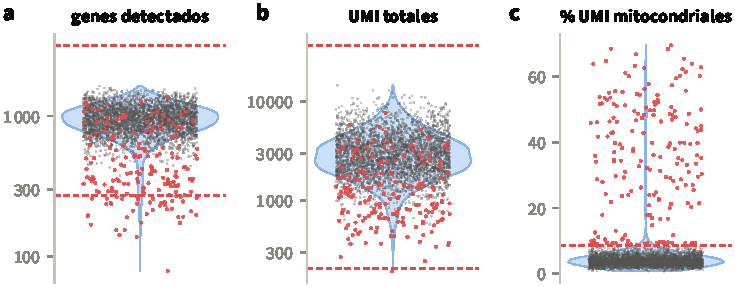
\includegraphics[width=\linewidth]{figuras/cap12/qc_violines.pdf}
\caption[Violines de control de calidad]{Métricas de QC de los \num{3360} códigos de barras con célula de la simulación: \num{3000} células sanas, 150 células dañadas y 210 dobletes. Cada punto es una célula; las líneas rojas discontinuas son los umbrales adaptativos (\cref{eq:12-mad}): 5 MAD sobre la escala logarítmica para genes \textbf{(a)} y UMI \textbf{(b)}, y la mediana más 3 MAD, \SI{8.52}{\percent}, para la fracción mitocondrial \textbf{(c)}. En rojo, las 185 células descartadas: las 150 dañadas y 35 sanas del extremo inferior. Obsérvese que la cola de células dañadas se ve con claridad en \textbf{c} pero se confunde con las células sanas pequeñas en \textbf{a} y \textbf{b}, y que ningún doblete supera los umbrales superiores: el QC univariante no los detecta.}
\label{fig:12-qc}
\end{figure}

\begin{ejemplo}{QC adaptativo sobre la simulación}{qc}
En los \num{3360} códigos con célula, la mediana es de \num{2763} UMI, 933 genes y \SI{3.89}{\percent} mitocondrial, y el MAD de $\log N$ vale \num{0.519}. Los umbrales resultan: UMI entre 205 y \num{37117}, genes entre 274 y \num{3171}, y porcentaje mitocondrial menor que \SI{8.52}{\percent}. Se descartan las 150 células dañadas (el \SI{100}{\percent}) y 35 de las \num{3000} sanas (\SI{1.2}{\percent}), y quedan \num{3175}. Pero los 210 dobletes pasan todos: una célula doble no es anómala en ninguna métrica por separado, porque la variabilidad natural del tamaño de las células (unas tres veces entre monocitos y linfocitos) cubre el aumento de UMI.
\end{ejemplo}

\begin{cuidado}[Los umbrales dependen del tejido]
No existe un porcentaje mitocondrial «correcto». Los cardiomiocitos, los hepatocitos o las células renales tienen de forma natural una alta carga mitocondrial, y un umbral del \SI{5}{\percent} copiado de un tutorial de sangre eliminaría precisamente las células de interés. Del mismo modo, una población rara de células pequeñas (neutrófilos, plaquetas) puede caer por debajo del umbral inferior de genes. Mire siempre las distribuciones por muestra, descarte con umbrales permisivos y revise después si algún \ingles{cluster} está definido solo por métricas de calidad.
\end{cuidado}

\subsection{Dobletes}

Los dobletes \emph{heterotípicos} (dos tipos celulares distintos) son peligrosos porque parecen un estado intermedio, o un tipo celular nuevo, que no existe. Los \emph{homotípicos} (dos células del mismo tipo) son casi indistinguibles de una célula grande, pero también mucho menos dañinos. Scrublet \parencite{c12-wolock2019} ataca el problema con una idea sencilla: si no sabemos cómo es un doblete real, fabriquemos dobletes artificiales sumando los perfiles de pares de células elegidas al azar, y preguntemos a cada célula observada cuántos de sus vecinos más cercanos son artificiales. Si en el espacio combinado hay $r$ dobletes simulados por cada célula observada y $q_c$ es la fracción de vecinos simulados de la célula $c$, la puntuación ajustada por la tasa esperada $\rho$ es
\begin{equation}\label{eq:12-scrublet}
s_c = \frac{q_c\,\rho/r}{1-\rho-q_c\,(1-\rho-\rho/r)}.
\end{equation}
\begin{simbolos}
\simbolo{$q_c$}{Fracción de los $k$ vecinos más cercanos de $c$ que son dobletes simulados.}
\simbolo{$r$}{Razón entre el número de dobletes simulados y el de células observadas.}
\simbolo{$\rho$}{Tasa de dobletes esperada, fijada según la carga del experimento (\cref{eq:12-poisson}).}
\simbolo{$s_c$}{Probabilidad estimada de que $c$ sea un doblete (puntuación de Scrublet).}
\end{simbolos}
La \cref{eq:12-scrublet} es la regla de Bayes: la densidad de dobletes simulados alrededor de $c$ (corregida por $r$) frente a la de singletes observados, con $\rho$ como probabilidad previa.

\begin{figure}[t]
\centering
\begin{tikzpicture}
\begin{axis}[curso, width=0.86\linewidth, height=5.2cm, ymode=log,
   xlabel={puntuación de doblete $s_c$}, ylabel={número de células},
   xmin=0, xmax=1, ymin=0.7, ymax=5000, legend pos=north east,
   unbounded coords=jump, /pgf/number format/1000 sep={\,}]
  \addplot[const plot mark mid, azul, very thick, fill=azul, fill opacity=0.12]
     table[x=x, y expr={\thisrow{ok}>0 ? \thisrow{ok} : nan}] {figuras/cap12/dobletes.dat};
  \addlegendentry{singletes (verdad simulada)}
  \addplot[const plot mark mid, naranja, very thick]
     table[x=x, y expr={\thisrow{dob}>0 ? \thisrow{dob} : nan}] {figuras/cap12/dobletes.dat};
  \addlegendentry{dobletes reales}
  \addplot[const plot mark mid, gris, thick, dashed]
     table[x=x, y expr={\thisrow{sim}>0 ? \thisrow{sim} : nan}] {figuras/cap12/dobletes.dat};
  \addlegendentry{dobletes simulados ($\div r$)}
  \draw[rojo, dashed, thick] (axis cs:0.25,0.7) -- (axis cs:0.25,5000);
  \node[etiqueta, text=rojooscuro, anchor=west] at (axis cs:0.26,2000) {umbral $0{,}25$};
\end{axis}
\end{tikzpicture}
\caption[Detección de dobletes al estilo Scrublet]{Distribución de la puntuación de doblete (\cref{eq:12-scrublet}) en las \num{3175} células que superaron el QC, con $k=28$ vecinos, $r=2$ y $\rho=\num{0.07}$. Los singletes se concentran cerca de cero (mediana \num{0.027}); los dobletes simulados (gris) muestran una distribución ancha que marca dónde caen los dobletes reales. Con un umbral de $0{,}25$ se detecta el \SI{40.9}{\percent} de los dobletes heterotípicos y solo el \SI{12.8}{\percent} de los homotípicos, a costa de marcar el \SI{0.51}{\percent} de los singletes. La detección es imperfecta, pero elimina justamente los dobletes que más engañan: los que unen tipos celulares distantes. Escala vertical logarítmica.}
\label{fig:12-dobletes}
\end{figure}

\subsection{Normalización}

Dos células idénticas pueden producir librerías de tamaño muy distinto: la eficiencia de captura y de transcripción inversa varía de una gota a otra. Antes de comparar células hay que eliminar esa variación técnica, sin borrar la biológica. El modelo de partida para las cuentas de UMI es la binomial negativa (BN), el mismo modelo gamma-Poisson del \cref{cap:11}:
\begin{equation}\label{eq:12-nb}
x_{cg}\sim\mathrm{BN}(\mu_{cg},\theta_g),\qquad \mu_{cg}=s_c\,q_{g,t(c)},\qquad \Var[x_{cg}]=\mu_{cg}+\frac{\mu_{cg}^2}{\theta_g},\qquad \Prob(x_{cg}=0)=\left(\frac{\theta_g}{\theta_g+\mu_{cg}}\right)^{\theta_g}.
\end{equation}
\begin{simbolos}
\simbolo{$s_c$}{Factor de tamaño de la célula $c$: eficiencia técnica global de su librería.}
\simbolo{$q_{g,t(c)}$}{Expresión del gen $g$ en el estado biológico $t(c)$ de la célula.}
\simbolo{$\theta_g$}{Parámetro de dispersión inversa; $\theta\to\infty$ recupera la Poisson.}
\end{simbolos}
Un punto que costó años aclarar: los muchos ceros de los datos de gotas \emph{no} requieren un modelo con inflación de ceros. \textcite{c12-svensson2020} comprobó, en experimentos de control con ARN sintético sin variación biológica, que la fracción de ceros observada es la que predice la BN con la media observada. Los ceros son, sobre todo, genes poco expresados muestreados con poca profundidad.

\paragraph{Normalización por tamaño de librería y logaritmo} El procedimiento por defecto en Scanpy estima $s_c\propto N_c$, escala cada célula a un total común (típicamente $10^4$, «cuentas por diez mil» o CP10k) y aplica un logaritmo desplazado:
\begin{equation}\label{eq:12-lognorm}
y_{cg} = \log\!\left(1 + \frac{x_{cg}}{N_c}\cdot 10^4\right).
\end{equation}
¿Por qué el logaritmo? Porque la varianza de las cuentas crece con la media, y los métodos posteriores (PCA, distancias euclídeas) dan más peso a los genes de mayor varianza. Por el método delta, si $X$ tiene media $\mu$ y varianza $\sigma^2$,
\begin{equation}\label{eq:12-delta}
\Var[\log(1+X)] \approx \frac{\sigma^2}{(1+\mu)^2} = \frac{\mu+\mu^2/\theta}{(1+\mu)^2}\;\xrightarrow{\;\mu\to\infty\;}\;\frac{1}{\theta}.
\end{equation}
Para genes muy expresados el logaritmo estabiliza la varianza en $1/\theta$, independiente de la media. Para genes poco expresados ($\mu\ll 1$) la varianza queda $\approx\mu$: la transformación no los estabiliza del todo, y el pseudoconteo 1 (arbitrario) influye en el resultado.

\begin{ejemplo}{Normalizar una célula}{norm}
Un monocito CD14 de la simulación tiene $N_c=\num{6359}$ UMI, 5 de ellos de \gen{LYZ}. Su valor normalizado es $5/\num{6359}\times10^4=\num{7.9}$ CP10k, y tras la \cref{eq:12-lognorm}, $y=\ln(1+\num{7.9})=\num{2.182}$. Un linfocito con la mitad de UMI y la misma proporción de \gen{LYZ} tendría exactamente el mismo $y$, que es lo que buscamos: la normalización compara proporciones, no cuentas.
\end{ejemplo}

\paragraph{Factores de tamaño por agrupamiento} Suponer $s_c\propto N_c$ equivale a suponer que todas las células tienen el mismo contenido total de ARN, lo cual es falso entre tipos celulares, y la estimación es muy ruidosa en células con pocas cuentas. El método de \textcite{c12-lun2016}, implementado en \texttt{scran}, suma las cuentas de grupos (\ingles{pools}) de células parecidas, donde hay pocos ceros y los cocientes de medianas son estables, estima un factor para cada grupo y recupera los factores individuales resolviendo un sistema lineal:
\begin{equation}\label{eq:12-pool}
\hat{S}_P = \operatorname*{med}_g \frac{\sum_{c\in P} x_{cg}}{\bar{x}_g}\;\approx\;\sum_{c\in P} s_c\qquad\text{para muchos grupos }P,
\end{equation}
con $\bar{x}_g$ la media del gen en una pseudocélula de referencia. Cada célula participa en varios grupos, de modo que hay más ecuaciones que incógnitas y el sistema se resuelve por mínimos cuadrados.

\paragraph{Residuos de Pearson (sctransform)} \textcite{c12-hafemeister2019} propusieron abandonar la división por $N_c$ y modelar la profundidad directamente. Para cada gen se ajusta una regresión BN con el logaritmo del tamaño de la librería como covariable, se regularizan los parámetros compartiendo información entre genes de expresión parecida, y se usan como datos normalizados los residuos de Pearson:
\begin{equation}\label{eq:12-pearson}
\log\mu_{cg} = \beta_{0g} + \beta_{1g}\log N_c,\qquad
r_{cg} = \frac{x_{cg}-\hat\mu_{cg}}{\sqrt{\hat\mu_{cg}+\hat\mu_{cg}^2/\hat\theta_g}}.
\end{equation}
\begin{simbolos}
\simbolo{$\beta_{0g},\beta_{1g}$}{Intercepto y pendiente de la regresión del gen $g$ sobre la profundidad.}
\simbolo{$\hat\mu_{cg}$}{Cuenta esperada si la célula solo difiriera de las demás en profundidad.}
\simbolo{$r_{cg}$}{Residuo de Pearson: desviación en unidades de desviación estándar del modelo.}
\end{simbolos}
Si el gen solo varía por razones técnicas, $r_{cg}$ tiene media 0 y varianza 1 en todas las células, sea cual sea la profundidad; la variación biológica aparece como exceso de varianza. Esta es la normalización por defecto de Seurat \parencite{c12-hao2021}.

\subsection{Genes altamente variables}

De unos \num{20000} genes, la mayoría no distingue tipos celulares: son genes constitutivos o genes apenas detectados cuya variación es ruido de muestreo. Restringir el análisis a los genes \emph{altamente variables} (HVG) reduce el ruido y el coste. El criterio no puede ser la varianza bruta, porque la varianza crece con la media; hay que comparar cada gen con los genes de expresión media similar. En el sabor clásico, se calcula la dispersión $d_g=\log(\sigma_g^2/\mu_g)$, se agrupan los genes en intervalos de media y dentro de cada intervalo se estandariza:
\begin{equation}\label{eq:12-hvg}
z_g = \frac{d_g - \operatorname{media}\{d_h : h\in B(g)\}}{\operatorname{de}\{d_h : h\in B(g)\}},
\end{equation}
con $B(g)$ el intervalo de medias al que pertenece $g$. Se retienen los genes de mayor $z_g$ (de \num{2000} a \num{5000} en datos reales).

\begin{figure}[t]
\centering
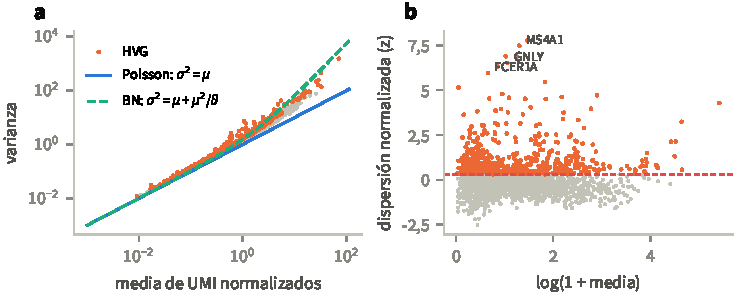
\includegraphics[width=\linewidth]{figuras/cap12/media_varianza.pdf}
\caption[Relación media-varianza y genes altamente variables]{\textbf{(a)} Varianza frente a media de las cuentas normalizadas por factor de tamaño para los \num{2000} genes simulados (escala log-log). La línea azul es la varianza de Poisson; la verde, una BN con la dispersión estimada por momentos. Casi todos los genes siguen la curva de ruido; los que la superan con creces (naranja) son los que varían entre tipos celulares. \textbf{(b)} Dispersión normalizada dentro de intervalos de media (\cref{eq:12-hvg}) frente a la expresión media. Los 500 genes por encima de la línea roja son los HVG; entre ellos están 31 de los 32 marcadores simulados y ningún gen mitocondrial.}
\label{fig:12-hvg}
\end{figure}

La \cref{fig:12-hvg} muestra el resultado en la simulación. Un detalle instructivo: la dispersión BN estimada por momentos con los datos normalizados de las células T CD4 vale $\hat\theta\approx\num{1.83}$, muy por debajo del valor simulado (mediana \num{6.02}). No es un error de cálculo: al dividir por un factor de tamaño aleatorio, las células pequeñas inflan la componente de Poisson de la varianza, y las cuentas normalizadas ya no son binomiales negativas. Es la razón de fondo por la que \textcite{c12-hafemeister2019} prefieren modelar la profundidad a dividir por ella.

\begin{codigo}[qc\_normalizacion.py]
import scanpy as sc

adata = sc.read_10x_h5("filtered_feature_bc_matrix.h5")
adata.var_names_make_unique()
adata.var["mt"] = adata.var_names.str.startswith("MT-")
sc.pp.calculate_qc_metrics(adata, qc_vars=["mt"],
                           percent_top=None, log1p=False,
                           inplace=True)
sc.pl.violin(adata, ["n_genes_by_counts", "total_counts",
                     "pct_counts_mt"], jitter=0.4, multi_panel=True)
ok = ((adata.obs.n_genes_by_counts > 250)
      & (adata.obs.pct_counts_mt < 8))
adata = adata[ok].copy()
sc.pp.filter_genes(adata, min_cells=3)
sc.pp.scrublet(adata)                    # Scanpy >= 1.10
adata = adata[~adata.obs["predicted_doublet"]].copy()
adata.layers["counts"] = adata.X.copy()  # cuentas crudas
sc.pp.normalize_total(adata, target_sum=1e4)
sc.pp.log1p(adata)
sc.pp.highly_variable_genes(adata, n_top_genes=2000,
                            flavor="seurat_v3", layer="counts")
\end{codigo}

\begin{cuidado}[El orden importa]
La selección de HVG con \texttt{flavor="seurat\_v3"} espera cuentas \emph{crudas} (por eso se guardan en una capa); los sabores \texttt{"seurat"} y \texttt{"cell\_ranger"} esperan datos log-normalizados. Scrublet debe ejecutarse sobre cuentas crudas y, si hay varias muestras, por separado en cada una, porque los dobletes solo pueden formarse dentro de un mismo canal.
\end{cuidado}

% ---------------------------------------------------------------------
\section{PCA, t-SNE y UMAP}\label{sec:12-reduccion}
% ---------------------------------------------------------------------
\enlacerepo{12.2 · PCA, t-SNE y UMAP}

\begin{intuicion}[Sombras chinescas]
Un titiritero proyecta en la pared la sombra de sus manos. De una misma mano, según cómo la gire frente a la lámpara, puede salir un conejo, un perro o un borrón irreconocible. Toda proyección pierde información; la cuestión es qué ángulo conserva lo que nos importa. Reducir la dimensión de los datos de célula única es buscar ese ángulo: pasar de miles de genes a dos coordenadas que quepan en una página. El PCA elige el ángulo en el que la sombra es más \emph{grande}; t-SNE y UMAP renuncian a la proyección rígida y moldean una sombra nueva en la que los vecinos siguen siendo vecinos, aunque las distancias largas dejen de significar algo.
\end{intuicion}

Después de la normalización tenemos una matriz de $n\approx\num{3000}$ células por \num{500} HVG. Cada célula es un punto en un espacio de 500 dimensiones. Pero los genes no varían de forma independiente: los programas transcripcionales mueven decenas de genes a la vez, así que la información está concentrada en un subespacio de dimensión mucho menor. La reducción de dimensión cumple dos papeles distintos que conviene no confundir: \emph{compresión} para el análisis (PCA, unas 30--50 dimensiones, sobre las que se calculan vecinos, grupos y trayectorias) y \emph{visualización} (t-SNE, UMAP, dos dimensiones, solo para mirar).

\subsection{Análisis de componentes principales}

Sea $Z\in\R^{n\times p}$ la matriz de expresión con cada gen centrado (y, habitualmente, escalado a varianza unitaria y truncado en $\pm10$ para que ningún gen domine). La matriz de covarianzas es $S=\frac{1}{n-1}Z^{\top}Z$. Buscamos la dirección unitaria $w$ en la que la proyección $Zw$ tiene varianza máxima:
\begin{equation}\label{eq:12-pca-prob}
\max_{w\in\R^p}\; w^{\top} S\, w \qquad\text{sujeto a}\qquad w^{\top}w = 1.
\end{equation}
Con el lagrangiano $\mathcal{L}(w,\lambda)=w^\top S w-\lambda(w^\top w-1)$ e igualando el gradiente a cero,
\begin{equation}\label{eq:12-pca-eig}
\nabla_w\mathcal{L}=2Sw-2\lambda w=0\;\Longrightarrow\; S\,w=\lambda\,w,\qquad w^\top S w=\lambda\,w^\top w=\lambda.
\end{equation}
\begin{simbolos}
\simbolo{$Z$}{Matriz células $\times$ genes centrada (y escalada).}
\simbolo{$S$}{Matriz de covarianzas entre genes, simétrica y semidefinida positiva.}
\simbolo{$w$}{Vector de cargas (\ingles{loadings}): peso de cada gen en la componente.}
\simbolo{$\lambda$}{Multiplicador de Lagrange; resulta ser la varianza capturada.}
\end{simbolos}
Los puntos críticos son los vectores propios de $S$, y la varianza capturada es el valor propio correspondiente: el máximo es el vector propio del mayor valor propio. Repitiendo el argumento con la restricción adicional de ortogonalidad a las direcciones ya encontradas se obtienen las siguientes componentes, en orden decreciente de $\lambda$. Como $S$ es simétrica, sus vectores propios son ortogonales y el procedimiento está bien definido. En la práctica no se forma $S$: se usa la descomposición en valores singulares $Z=U\Sigma V^\top$, de la que se lee todo a la vez.

\begin{teorema}{PCA mediante la SVD}{pca}
Si $Z = U\Sigma V^{\top}$ con $\sigma_1\ge\sigma_2\ge\cdots\ge0$, entonces las columnas de $V$ son las direcciones principales, las coordenadas de las células son $ZV = U\Sigma$, la varianza de la componente $k$ es $\lambda_k=\sigma_k^2/(n-1)$ y la fracción de varianza explicada es $\lambda_k/\sum_j\lambda_j$. Además, $U_k\Sigma_kV_k^{\top}$ (truncada a las $k$ primeras) es la mejor aproximación de rango $k$ de $Z$ en norma de Frobenius \parencite{c12-hastie2009}.
\end{teorema}

La última afirmación da la justificación estadística de usar las primeras componentes como entrada de todo lo que sigue: son la mejor compresión lineal posible, y las componentes de menor varianza, descartadas, contienen sobre todo ruido de muestreo. La derivación desde el punto de vista de la genética de poblaciones se discute en el \cref{cap:10}.

\paragraph{¿Cuántas componentes?} La \cref{fig:12-pca} muestra la varianza explicada en la simulación. Es poca en términos absolutos: PC1 explica el \SI{2.45}{\percent} y las 30 primeras, el \SI{15.2}{\percent}; el resto es ruido de Poisson, que se reparte en todas las direcciones. Para saber qué componentes contienen señal, comparamos con un modelo nulo en el que se permutan las células independientemente en cada gen, lo que destruye las correlaciones y conserva las distribuciones marginales. En los datos permutados ninguna componente supera el \SI{0.39}{\percent}; en los reales, siete sí, tantas como la estructura simulada (siete tipos celulares definen seis contrastes, más un estado continuo dentro de las células T CD4). En la práctica se usan 30--50 componentes; tomar de más es barato, tomar de menos puede fundir poblaciones raras.

\begin{figure}[t]
\centering
\begin{tikzpicture}
\begin{axis}[curso, width=0.86\linewidth, height=5.2cm,
   xlabel={componente principal}, ylabel={varianza explicada (\%)},
   xmin=0, xmax=51, ymin=0, ymax=2.7, legend pos=north east]
  \addplot[azul, very thick, mark=*, mark size=1.1pt] table[x=pc, y=frac] {figuras/cap12/pca_var.dat};
  \addlegendentry{datos}
  \addplot[gris, thick, dashed, mark=o, mark size=1pt] table[x=pc, y=frac] {figuras/cap12/pca_nulo.dat};
  \addlegendentry{nulo (genes permutados)}
  \draw[naranja, dashed] (axis cs:7.5,0) -- (axis cs:7.5,2.7);
  \node[etiqueta, text=naranja!80!black, anchor=west] at (axis cs:8,1.6) {7 PC por encima del nulo};
  \node[etiqueta, anchor=west, align=left] at (axis cs:2,2.45) {PC1: \gen{LYZ}, \gen{S100A9}, \gen{S100A8}, \gen{CD14}};
\end{axis}
\end{tikzpicture}
\caption[Varianza explicada por las componentes principales]{Gráfico de codo (\ingles{elbow plot}) de las 50 primeras componentes principales de los 500 HVG de la simulación, frente a un modelo nulo en el que cada gen se permuta de forma independiente. Las siete primeras componentes superan claramente al nulo; a partir de ahí la curva se aplana en una meseta de ruido. PC1 separa células mieloides de linfoides (sus mayores cargas son genes de monocitos), mientras que PC2 está dominada por los genes del estado continuo simulado dentro de las células T CD4.}
\label{fig:12-pca}
\end{figure}

\subsection{t-SNE: conservar vecindarios}

El PCA es lineal y global: preserva bien las grandes distancias y comprime los grupos pequeños unos sobre otros (\cref{fig:12-embeddings}a). El \ingles{t-distributed stochastic neighbor embedding} (t-SNE), propuesto por van der Maaten y Hinton en 2008 y popularizado en célula única, invierte la prioridad: renuncia a las distancias largas para conservar los vecindarios \parencite{c12-kobak2019}.

\paragraph{Similitudes en alta dimensión} Para cada célula $i$, t-SNE define una distribución de probabilidad sobre las demás, gaussiana en la distancia:
\begin{equation}\label{eq:12-tsne-p}
p_{j\mid i}=\frac{\exp\!\left(-\lVert x_i-x_j\rVert^2/2\sigma_i^2\right)}{\sum_{k\neq i}\exp\!\left(-\lVert x_i-x_k\rVert^2/2\sigma_i^2\right)},\qquad
\mathrm{Perp}(P_i)=2^{H(P_i)},\qquad H(P_i)=-\sum_{j}p_{j\mid i}\log_2 p_{j\mid i}.
\end{equation}
\begin{simbolos}
\simbolo{$x_i$}{Coordenadas de la célula $i$ en el espacio de entrada (p.\,ej., 30 PC).}
\simbolo{$\sigma_i$}{Ancho de banda propio de cada célula, elegido por bisección.}
\simbolo{$\mathrm{Perp}$}{Perplejidad: número efectivo de vecinos que «ve» cada célula; es el único parámetro que fija el usuario.}
\simbolo{$H(P_i)$}{Entropía de Shannon (en bits) de la distribución de vecinos de $i$.}
\end{simbolos}
El ancho $\sigma_i$ no es común: se ajusta en cada célula para que la perplejidad sea la deseada. Así, en regiones densas $\sigma_i$ es pequeño y en regiones dispersas es grande, y cada célula considera aproximadamente el mismo número de vecinos. Las probabilidades se simetrizan, $p_{ij}=(p_{j\mid i}+p_{i\mid j})/2n$.

\begin{ejemplo}{La perplejidad como número de vecinos}{perp}
Para una célula de la simulación, en el espacio de 30 PC, la bisección da $\sigma=\num{0.893}$ con perplejidad 5, $\sigma=\num{1.722}$ con 30 y $\sigma=\num{2.834}$ con 300. Con perplejidad 5, su vecino más cercano recibe el \SI{42.4}{\percent} de la probabilidad y solo 13 células superan la probabilidad uniforme $1/(n-1)$; con 300, el vecino más cercano recibe el \SI{2.5}{\percent} y 331 células superan ese nivel. Una perplejidad de $2^H$ equivale a la incertidumbre de elegir uniformemente entre $2^H$ vecinos.
\end{ejemplo}

\paragraph{Similitudes en baja dimensión y la cola pesada} En el mapa bidimensional $y_1,\dots,y_n$ las similitudes se miden con una distribución $t$ de Student con un grado de libertad (Cauchy):
\begin{equation}\label{eq:12-tsne-q}
q_{ij}=\frac{\left(1+\lVert y_i-y_j\rVert^2\right)^{-1}}{\sum_{k\neq l}\left(1+\lVert y_k-y_l\rVert^2\right)^{-1}}.
\end{equation}
¿Por qué no otra gaussiana? Por el \emph{problema de hacinamiento}: en 30 dimensiones caben muchos más puntos a distancia moderada de una célula que en un plano. Si forzamos a todos esos vecinos moderados a caber alrededor de ella en dos dimensiones, se amontonan. La cola pesada de la $t$ permite que los puntos moderadamente lejanos se coloquen mucho más lejos en el mapa sin penalización, lo que abre espacio y separa los grupos.

\begin{teorema}{Función de costo y gradiente de t-SNE}{tsne}
t-SNE minimiza la divergencia de Kullback-Leibler entre las similitudes de alta y baja dimensión,
\begin{equation}\label{eq:12-kl}
C=\mathrm{KL}(P\,\Vert\,Q)=\sum_{i\neq j}p_{ij}\log\frac{p_{ij}}{q_{ij}},
\end{equation}
cuyo gradiente respecto de la posición de la célula $i$ es
\begin{equation}\label{eq:12-grad}
\frac{\partial C}{\partial y_i}=4\sum_{j\neq i}\left(p_{ij}-q_{ij}\right)\left(y_i-y_j\right)\left(1+\lVert y_i-y_j\rVert^2\right)^{-1}.
\end{equation}
\end{teorema}
La \cref{eq:12-grad} se lee como un sistema de resortes: si $p_{ij}>q_{ij}$ (las células son más vecinas en el espacio original que en el mapa) el término atrae a $y_i$ hacia $y_j$; si $p_{ij}<q_{ij}$, las repele. La KL es asimétrica, y esa asimetría es la esencia del método: poner lejos a dos vecinos reales (grande $p$, pequeño $q$) cuesta mucho; poner cerca a dos células lejanas (pequeño $p$, grande $q$) cuesta poco. t-SNE conserva vecindarios y deja libres las distancias largas.

\begin{figure}[t]
\centering
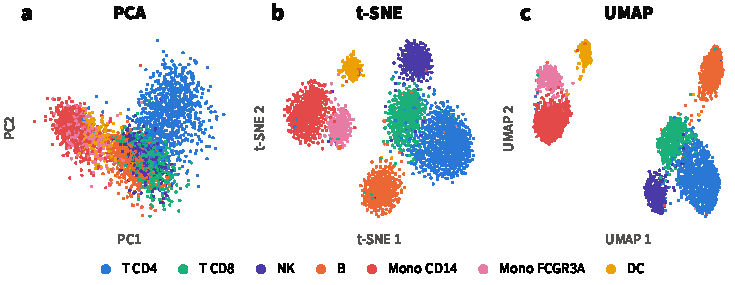
\includegraphics[width=\linewidth]{figuras/cap12/embeddings.pdf}
\caption[PCA, t-SNE y UMAP sobre los mismos datos]{Las \num{3085} células que superaron el QC, representadas con tres métodos a partir de las mismas 30 componentes principales y coloreadas por el tipo celular \emph{simulado} (que ningún método conoce). \textbf{(a)} Las dos primeras PC separan el eje mieloide-linfoide y el estado continuo de las células T CD4, pero superponen tipos que difieren en direcciones de menor varianza. \textbf{(b)} t-SNE (perplejidad 30, inicialización PCA) separa los siete tipos en islas compactas. \textbf{(c)} UMAP ($k=15$, \texttt{min\_dist}$=\num{0.3}$) produce grupos similares, más compactos y con más espacio vacío entre ellos. Ni el tamaño de las islas ni la distancia entre ellas deben leerse al pie de la letra (\cref{fig:12-distancias}).}
\label{fig:12-embeddings}
\end{figure}

\paragraph{La perplejidad cambia la imagen} La \cref{fig:12-perp} muestra el efecto del único parámetro de t-SNE. Con perplejidad baja, cada célula solo atiende a un puñado de vecinos y los grupos se fragmentan en subgrupos espurios; con perplejidad alta, el mapa conserva mejor la estructura global, pero los tipos cercanos (monocitos CD14 y FCGR3A; linfocitos T CD4 y CD8) se funden. \textcite{c12-kobak2019} recomiendan inicializar con PCA (para heredar la estructura global en lugar de partir de posiciones aleatorias), usar una perplejidad del orden de $n/100$ en conjuntos grandes o combinar varias escalas, y aumentar la «exageración» de las atracciones al inicio. Para millones de células, FIt-SNE acelera el cálculo interpolando las fuerzas repulsivas en una rejilla \parencite{c12-linderman2019}.

\begin{figure}[t]
\centering
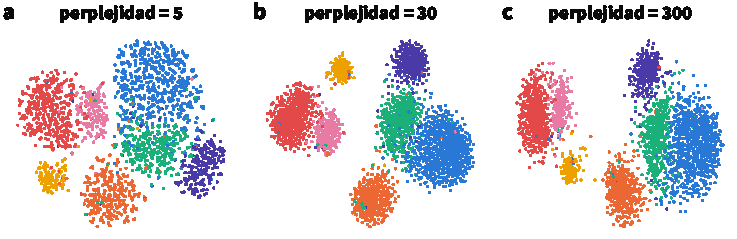
\includegraphics[width=\linewidth]{figuras/cap12/perplejidad.pdf}
\caption[Efecto de la perplejidad en t-SNE]{t-SNE de los mismos datos con perplejidades 5, 30 y 300 (misma semilla, inicialización PCA). \textbf{(a)} Con perplejidad 5 las islas se ven granuladas: cada célula solo «ve» a unos pocos vecinos y aparecen agrupamientos locales sin significado biológico. \textbf{(b)} El valor por defecto, 30. \textbf{(c)} Con perplejidad 300 (el \SI{10}{\percent} de las células) la disposición global es más fiel a las relaciones entre linajes, pero los tipos emparentados se funden. No hay una perplejidad «correcta»: conviene mirar varias.}
\label{fig:12-perp}
\end{figure}

\subsection{UMAP: un grafo difuso}

UMAP (\ingles{uniform manifold approximation and projection}) parte de la teoría de conjuntos difusos y la topología algebraica, pero su algoritmo se parece mucho a t-SNE \parencite{c12-mcinnes2018}. Primero construye un grafo de $k$ vecinos más cercanos con pesos
\begin{equation}\label{eq:12-umap-v}
v_{j\mid i}=\exp\!\left(-\frac{d(x_i,x_j)-\rho_i}{\sigma_i}\right),\qquad \sum_{j=1}^{k} v_{j\mid i}=\log_2 k,\qquad v_{ij}=v_{j\mid i}+v_{i\mid j}-v_{j\mid i}\,v_{i\mid j},
\end{equation}
\begin{simbolos}
\simbolo{$\rho_i$}{Distancia de $i$ a su vecino más cercano: garantiza que toda célula tenga al menos un vecino con peso 1.}
\simbolo{$\sigma_i$}{Escala local, elegida para que la suma de pesos sea $\log_2 k$ (análoga a la perplejidad).}
\simbolo{$v_{ij}$}{Peso simétrico de la arista: la probabilidad de que exista al menos una de las dos aristas dirigidas (unión difusa).}
\simbolo{$k$}{Número de vecinos (\texttt{n\_neighbors}); controla el equilibrio entre estructura local y global.}
\end{simbolos}
y después busca coordenadas $y_i$ cuyas similitudes $w_{ij}=(1+a\lVert y_i-y_j\rVert^{2b})^{-1}$ se parezcan a $v_{ij}$, minimizando la entropía cruzada
\begin{equation}\label{eq:12-umap-ce}
\mathrm{CE}=\sum_{i\neq j}\left[v_{ij}\log\frac{v_{ij}}{w_{ij}}+\left(1-v_{ij}\right)\log\frac{1-v_{ij}}{1-w_{ij}}\right].
\end{equation}
El primer término es el atractivo de t-SNE; el segundo, ausente en la KL, penaliza explícitamente colocar cerca a células que no son vecinas. Los parámetros $a$ y $b$ se ajustan a partir de \texttt{min\_dist}, que fija lo compactos que se permite que queden los grupos. Como las similitudes no se normalizan globalmente, la optimización se puede hacer por descenso de gradiente estocástico muestreando aristas, lo que la hace muy rápida. \textcite{c12-becht2019} mostraron en datos de citometría y de célula única que UMAP es más rápido que las implementaciones de t-SNE de entonces y que representa mejor la continuidad entre poblaciones; análisis posteriores atribuyeron buena parte de la diferencia en estructura global a la inicialización más que al algoritmo \parencite{c12-kobak2019}.

\subsection{Lo que un embedding no dice}

Un mapa bidimensional es una herramienta de exploración, no una medida. La \cref{fig:12-distancias} cuantifica la advertencia con la simulación: para \num{4000} pares de células al azar comparamos su distancia en el espacio de 30 PC con su distancia en el mapa.

\begin{figure}[t]
\centering
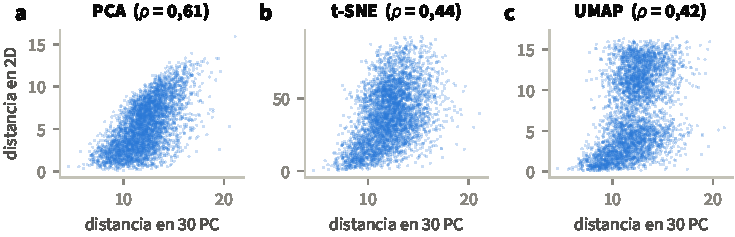
\includegraphics[width=\linewidth]{figuras/cap12/distancias.pdf}
\caption[Distorsión de distancias en los embeddings]{Distancia entre \num{4000} pares de células al azar en el espacio de 30 PC (horizontal) frente a su distancia en cada mapa bidimensional (vertical), con la correlación de Spearman $\rho$. El PCA en 2D conserva mejor el orden de las distancias ($\rho=\num{0.61}$) pero es una mala representación local: solo el \SI{4.3}{\percent} de los 15 vecinos de cada célula siguen siéndolo en el plano. t-SNE ($\rho=\num{0.44}$) y UMAP ($\rho=\num{0.42}$) conservan más vecinos (\SI{23.3}{\percent} y \SI{11.9}{\percent}), pero la relación entre distancias reales y aparentes es no monótona: a igual distancia real, dos pares pueden quedar en el mismo grupo del mapa o en extremos opuestos.}
\label{fig:12-distancias}
\end{figure}

\textcite{c12-chari2023} llevaron el argumento al extremo: mostraron que los \ingles{embeddings} de t-SNE y UMAP distorsionan severamente las distancias de conjuntos de datos reales, y que se puede forzar a que los datos adopten casi cualquier forma deseada (incluso la de un elefante) conservando niveles de preservación de vecindarios comparables. La lección práctica es una lista de prohibiciones:

\begin{itemize}
  \item \textbf{No interprete tamaños.} t-SNE y UMAP adaptan la escala local a la densidad; un grupo grande en el mapa no es un grupo más heterogéneo.
  \item \textbf{No interprete distancias entre grupos.} En nuestra simulación, la correlación entre las distancias de los centroides de los siete tipos en el espacio de PC y en el mapa es de \num{0.835} para t-SNE y \num{0.801} para UMAP: el orden se conserva en gran parte, pero no la magnitud.
  \item \textbf{No cuantifique en 2D.} Agrupamientos, trayectorias y distancias se calculan en el espacio de PC (o en el grafo de vecinos), nunca en las coordenadas del mapa.
\end{itemize}

\begin{ideaclave}
PCA para calcular; t-SNE y UMAP para mirar. Un vecino en el mapa es probablemente un vecino real; una distancia en el mapa no es una distancia.
\end{ideaclave}

\begin{codigo}[reduccion.py]
sc.pp.scale(adata, max_value=10)           # z-score, truncado en 10
sc.tl.pca(adata, n_comps=50, mask_var="highly_variable")
sc.pl.pca_variance_ratio(adata, n_pcs=50, log=True)
sc.pp.neighbors(adata, n_neighbors=15, n_pcs=30)   # grafo kNN
sc.tl.umap(adata, min_dist=0.3)
sc.tl.tsne(adata, n_pcs=30, perplexity=30)
sc.pl.umap(adata, color=["CD3E", "MS4A1", "LYZ", "pct_counts_mt"])
\end{codigo}

\begin{cuidado}[UMAP necesita el grafo]
En Scanpy, \texttt{sc.tl.umap} no recalcula vecinos: usa el grafo de \texttt{sc.pp.neighbors}. Cambiar \texttt{n\_neighbors} en el grafo cambia a la vez el mapa y los \ingles{clusters} de la sección siguiente. Colorear el mapa por \texttt{pct\_counts\_mt} o \texttt{total\_counts} es la forma más rápida de descubrir que un «tipo celular nuevo» es en realidad un grupo de células de mala calidad.
\end{cuidado}

%%PARTE2%%
